\documentclass[../main.tex]{subfiles}

\begin{document}
\chapter{Stetige Funktionen}

\section{Stetigkeit}

Folgende Definition von Weierstrass
ist aus gutem Grund sehr berühmt.

\begin{definition}
  Sei $A \subset \mathbb{R}$ 
  eine beliebige Teilmenge.
  Eine Funktion
  $f \colon A \to \mathbb{R}$ 
  heisst \emph{stetig} im Punkt
  $p \in A$, falls für
  alle vorgegebenen $\varepsilon > 0$
  ein  $\delta > 0$ existiert,
  so dass für alle $q \in A$ 
  mit $|q-p| \leq \delta$ gilt,
  dass $|f(q) - f(p)| \leq \varepsilon$.
  Falls $f \colon A \to \mathbb{R}$ in
  allen Punkten $p \in A$ stetig ist,
  dann heisst $f$ \emph{stetig}.
\end{definition}

\begin{figure}[htb]
  \centering
  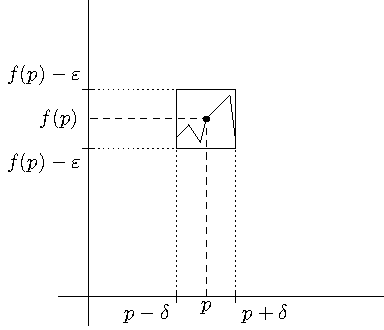
\includegraphics{chapter3/images/conti}
  \caption{Stetigkeit bedeutet, dass der Graph
  der Funktion den Rand des eingezeichneten Rechtecks
nur rechts und links, aber nicht oben und unten
durchdringt.}%
  \label{fig:conti}
\end{figure}


\begin{examples}
  \leavevmode
  \begin{enumerate}[(1)]
    \item Die Identitätsfunktion
      \begin{align*}
        f \colon \mathbb{R} & \to \mathbb{R} \\
        p & \mapsto p
      \end{align*}
      ist stetig. Sei dazu $p \in \mathbb{R}$ fest
      und $\varepsilon > 0$ vorgegeben.
      Setze $\delta = \varepsilon$. Dann gilt
      für alle $q \in \mathbb{R}$ mit
      $|q - p| \leq \delta$, dass
      $|f(q) - f(p)| = |q - p| \leq \delta = \varepsilon$.
    \item Sei
      \[
        f(x) = 
        \begin{cases}
          0 & \text{falls } x \leq 0, \\
          1 & \text{falls } x > 0,
        \end{cases}
      \]
      siehe Abbildung~\ref{fig:jump}.
      Dann ist $f$ in allen Punkten ausser dem
      Nullpunkt stetig.
      Tatsächlich, sei $p \neq 0$
      und $\varepsilon > 0$ 
      vorgegeben.
      Setze $\delta = |p|/2 > 0$.
      Dann gilt für alle $q \in \mathbb{R}$ 
      mit $|q - p| \leq \delta$, dass
      $|f(q) - f(p)| = 0 \leq \varepsilon$.
      
      Sei nun $p = 0$. Betrachte $\varepsilon = 1/2$.
      Sei $\delta > 0$ beliebig.
      Dann gilt für $q = \delta/2$, dass
      $|q - p| = \delta/2 < \delta$.
      Es folgt
      \[
        |f(q) - f(p)| = |1 - 0| = 1 > \varepsilon.
      \]
      \begin{figure}[htb]
        \centering
      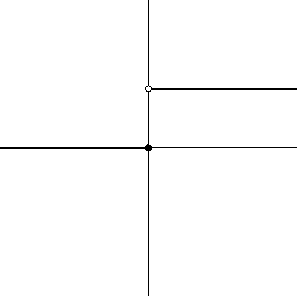
\includegraphics{chapter3/images/jump}
        \caption{Sprungstelle}%
        \label{fig:jump}
      \end{figure}

    \item Sei
      \[
        f(x) = 
        \begin{cases}
          1, & \text{falls } x \in \mathbb{Q}, \\
        0,& \text{falls } x \in \mathbb{R} \setminus \mathbb{Q}
        \end{cases}
      \]
      die \emph{Dirichletfunktion}.
      Dann ist $f$ in keinem Punkt stetig.
      Betrachte dazu $\varepsilon = 1/2$.
      Sei $p \in \mathbb{Q}$, das heisst $f(p) = 1$.
      Für alle $\delta > 0$ finden wir eine
      irrationale Zahl
      $q \in \mathbb{R} \setminus \mathbb{Q}$ mit
      $|q - p| \leq \delta$ 
      und
      $|f(q) - f(p)| = 1 > \varepsilon$.
      Tatsächlich, wähle $N \in \mathbb{N}$ 
      mit $\sqrt 2 / N \leq \delta$.
      Setze
      $q = p +\sqrt 2/N$. Dann gilt  $q \notin \mathbb{Q}$,
      also $f(q) = 0$.

      Analog, sei $p \in \mathbb{R} \setminus \mathbb{Q}$,
      das heisst $f(p) = 0$.
      Für alle $\delta > 0$ finden wir
      eine Zahl $q \in \mathbb{Q}$ mit $|q - p| \leq \delta$ 
      und
      $|f(q) - f(p)| = 1 > \varepsilon$.
      Tatsächlich,
      wähle $N \in \mathbb{N}$ mit $1/N \leq \delta$.
      Dann existiert $a \in \mathbb{Z}$
      so dass
      $|a/N - p| \leq 1/N$.
      Setze $q = a/N$.
    \item Sei $f(x) = x^n$ für $n \in \mathbb{N}$.
      Dann ist $f$ stetig auf $\mathbb{R}$.
      Sei also $p \in \mathbb{R}$ vorgegeben und
      sei $\varepsilon > 0$.
      Für
      $h \in \mathbb{R}$ mit $|h| \leq 1$ gilt
      \[
        f(x + h) = (x + h)^n = \sum_{k=0}^{n} \binom{n}{k}
        x^{n-k}h^k
        = x^n + nx^{n-1}h + \frac{n(n-1)}{2}x^{n-2}h^2 + \cdots.
      \]
      Es folgt, dass
      \[
        |f(x + h) - f(x)| \leq |h| \cdot
        \left| \sum_{k=1}^{n} \binom{n}{k} x^{n-k} \right|,
      \]
      da $|h| \leq 1$.
      Setze jetzt
      \[
        \delta_1 = \frac{\varepsilon}{t+1},
      \]
      wobei
      \[
        t = \sum_{k=1}^{n} \binom{n}{k} |p|^{n-k},
      \]
      und $\delta = \min \{1, \delta_1\} > 0$.
      Für alle  $h \in \mathbb{R}$
      mit $|h| \leq \delta$ gilt also
      \[
        |f(p+h) - f(p)| \leq |h| \cdot t \leq
        \delta_1 \cdot t = \varepsilon \cdot \frac{t}{t+1}
        \leq \varepsilon.
      \]
      Also ist $f$ stetig im Punkt $p$.
    \item Betrachte die Funktion
      \begin{align*}
        f \colon \mathbb{R} \setminus \{0\} & \to \mathbb{R} \\
        x & \mapsto 1/x.
      \end{align*}
      Dann ist $f$ stetig in allen Punkten
      $p \in \mathbb{R} \setminus \{0\}$. Dies ist
      mühsam von Hand zu zeigen. Deshalb
      verwenden wir folgendes Lemma.
  \end{enumerate}
\end{examples}

\begin{lemma*}
  Sei $A \subset \mathbb{R}$ und seien
  $f, g \colon A \to \mathbb{R}$ im Punkt
  $p \in A$ stetig. Dann sind die Funktionen
  $f + g$ und $f \cdot g$ 
  im Punkt $p$ stetig.
  Falls $f(p) \neq 0$, dann
  existiert $a > 0$, so dass
  die Funktion $1/f$ auf der Menge
  $(p- a, p + a) \cap A$ definiert und 
  im Punkt $p$ stetig ist.
\end{lemma*}

\begin{proof}
  Als erstes zeigen wir,
  dass $f  + g$ stetig ist.
  Sei $\varepsilon > 0$ vorgegeben.
  Wähle $\delta_f > 0$ und  $\delta_g > 0$ 
  so dass für alle $q \in A$ mit
  $|q - p| \leq \delta_f$ gilt, dass
  $|f(q) - f(p)| \leq \varepsilon/2$,
  und so dass für alle
  $q \in A$ mit $|q - p| \leq \delta_g$ 
  git, dass
  $|g(p) - g(q)| \leq \varepsilon/2$.
  Setze $\delta = \min \{\delta_f, \delta_g\}$.
  Dann gilt für alle $q \in A$ mit
  $|q - p| \leq \delta$, dass
  \begin{align*}
  |(f + g)(q) - (f + g)(p)| &     = |f(q) + g(q) - f(p) - g(p)|\\
                            & \leq |f(q) - f(p)| + |g(q) - g(p)|\\
                            & \leq \varepsilon/2 + \varepsilon/2\\
                            &= \varepsilon.
  \end{align*}

  Wir zeigen nun, dass $f \cdot g$ stetig ist.
  Berechne
  \begin{align*}
     |(f\cdot g)(q) - (f \cdot g)(p)|
     & = |f(q) \cdot g(q) - f(p) \cdot g(p)| \\
     & = |f(q)g(q) - f(p)g(q) + f(p)g(q) - f(p) g(p)| \\
     & \leq |g(q)| \cdot |f(q) - f(p)| + 
     |f(p)| \cdot |g(q) - g(p)| \\
  \end{align*}
  Wähle $\delta_1 > 0$ so, dass immer wenn
  $|q - p| \leq \delta_1$ gilt, dann auch
  $|g(q) - g(p)| \leq 1$. Wähle
  $\delta_2 > 0$ so, dass immer
  wenn $|q - p| \leq \delta_2$ gilt, dann auch
  \[
    |f(q) - f(p)| \leq \frac{\varepsilon}{2} \cdot
    \frac{1}{|g(p)| + 1}.
  \]
  Wähle weiterhin $\delta_3 > 0$ so, dass immer wenn
  $|q - p| \leq \delta_3$ gilt, dann auch
  \[
    |g(q) - g(p)| \leq \frac{\varepsilon}{2} \cdot
    \frac{1}{|f(p)| + 1}.
  \]
  Setze $\delta = \min \{\delta_1, \delta_2, \delta_3 \}$.
  Für $q \in A$ mit $|q - p| \leq \delta$ gilt dann:
  \begin{align*}
    |(f \cdot g)(q) - (f \cdot g)(p)
    &\leq |g(q)| \cdot \frac{\varepsilon}{2} \cdot  
    \frac{1}{|g(p)| + 1}
    + |f(p)| \cdot \frac{\varepsilon}{2}
    \cdot \frac{1}{|f(p)| + 1}\\
    & \leq (|g(p)| + 1) \frac{\varepsilon}{2}
    \cdot \frac{1}{|g(p)| + 1} + \frac{\varepsilon}{2}  \\
    &= \varepsilon.
  \end{align*}
  
  Zuletzt behandeln wir $1/f$.
  Sei $p \in A$ mit $f(p) \neq 0$.
  Dann existiert nach Stetigkeit von
  $f$ im Punkt $p$ eine Zahl $a > 0$, so dass
  wenn $|q - p| \leq a$ gilt,
  dann auch
  \[
  |f(q) - f(p)| \leq \frac{|f(p)|}{2}.
  \]
  Also ist $1/f$ auf der Menge $(p-a, p+a) \cap A$ definiert,
  da dort $|f(q)| > 0$.
  Sei nun $\varepsilon > 0$. 
  Berechne
   \begin{align*}
     \left| \frac{1}{f(q)} - \frac{1}{f(p)} \right| 
     & = \left| \frac{f(p) - f(q)}{f(q)f(p)} \right| \\
     & \leq 2 \cdot \frac{|f(p) - f(q)|}{|f(p)|^2}. 
  \end{align*}
  Wähle $\delta > 0$, so dass $\delta \leq a$ 
  und immer wenn $|q - p| \leq \delta$,
  dann auch 
  \[
    |f(q) - f(p)| \leq \frac{\varepsilon}{2} \cdot |f(p)|^2.
  \]
  Es folgt für $q \in A$ mit $|q - p| \leq \delta$, dass
  \[
    \left| \frac{1}{f(q)}- \frac{1}{f(p)} \right|
    \leq 2 \cdot \frac{|f(p) - f(q)|}{|f(p)|^2} \leq \varepsilon.
    \qedhere
  \]
\end{proof}

\begin{applications}
  \leavevmode
  \begin{enumerate}[(1)]
    \item Alle Funktionen der Form
      \[
        f(x) = a_n x^n + a_{n-1} x^{n-1} + \cdots + a_{1} x + a_0,
      \]
      sogenannte \emph{Polynome},
      mit Koeffizienten $a_k \in \mathbb{R}$ sind stetig
      auf $\mathbb{R}$, da die Funktion $x \mapsto x$
      und konstante Funktionen stetig sind.
    \item Die Funktion $f(x) = 1/x$ ist stetig
      auf $\mathbb{R} \setminus \{0\}$.
  \end{enumerate}
\end{applications}

\subsection*{Folgenstetigkeit}
\begin{theorem}
  Sei $A \subset \mathbb{R}$ eine Teilmenge.
  Eine Funktion $f \colon A \to \mathbb{R}$ ist
  genau dann stetig im Punkt
  $p \in A$, wenn für alle
  konvergenten Folgen $a \colon \mathbb{N} \to A$
  mit $\lim_{n \to \infty}a_n = p$ gilt, dass
  \[
    \lim_{n \to \infty} f(a_n) = f(p).
  \]
\end{theorem}

\begin{proof}
  Für die Hinrichtung ``$\Rightarrow$'' sei $f$
  im Punkt $p$ stetig. Sei ${(a_{n})}_{n \in \mathbb{N}}$ 
  eine Folge in $A$ mit
  \[
    \lim_{n \to \infty} a_n = p.
  \]
  Sei $\varepsilon > 0$ vorgegeben.
  Dann existiert $\delta > 0$ so dass immer wenn
  $|q - p| \leq \delta$, dann auch
  $|f(q) - f(p)| \leq \varepsilon$.
  Wähle $N \in \mathbb{N}$, so
  dass für $n \in \mathbb{N}$ mit $n \geq N$ gilt,
  dass $|a_n - p| \leq \delta$.
  Es gilt also für $n \geq N$, dass
  $|f(a_n) - f(p)| \leq \varepsilon$.
  Also gilt
  \[
    \lim_{n \to \infty} f(a_n) = f(p).
  \]
  
  Für die Rückrichtung ``$\Leftarrow$'', nehme an,
  dass $f$ \emph{folgenstetig} in $p$ ist,
  das heisst dass für alle
  konvergenten Folgen $a \colon \mathbb{N} \to A$
  mit $\lim_{n \to \infty} a_n = p$ gilt,
  dass
  \[
    \lim_{n \to \infty} f(a_n) = f(p).
  \]
  Wir beweisen durch Widerspruch, dass
  $f$ stetig in $p$ ist.
  Nehme an, dass $f$ nicht stetig in $p$ ist.
  Dann existiert $\varepsilon_0 > 0$, so dass
  für alle $\delta > 0$ ein $q \in A$ 
  existiert, so dass
  $|q - p| \leq \delta$ und $|f(q) - f(p)| > \varepsilon_0$.
  Wähle nun eine Folge
  ${(a_{n})}_{n \in \mathbb{N}}$ wie folgt.
  Wähle $a_n \in A$ so dass
  $|a_n - p| \leq 1/(n+1)$ und $|f(a_n) - f(p)| > \varepsilon_0$.
  Nach Konstruktion gilt
  $\lim_{n \to \infty} a_n = p$, aber
  \[
    \lim_{n \to \infty} f(a_n) \neq f(p).
  \]
  Dies widerspricht der Folgenstetigkeit von $f$.
\end{proof}

Dieser Satz sagt, dass genau dann die Formel
\[
  \lim_{n \to \infty}  f(a_n) = f\left(\lim_{n \to \infty} a_n\right)
\]
gilt, wenn $f$ stetig ist.

\begin{application}
  Seien $f \colon A \to \mathbb{R}$ und $g \colon B \to \mathbb{R}$
  Funktionen mit $f(A) \subset B$. Falls $f$ im Punkt $p \in A$ 
  stetig ist, und $g$ im Punkt $f(p) \in B$ stetig ist,
  dann ist $g \circ f\colon A \to \mathbb{R}$ im Punkt $p$ stetig.
\end{application}

\begin{proof}
  Wir verwenden die Folgenstetigkeit um einen schnellen
  Beweis zu liefern.
  Sei  ${(a_{n})}_{n \in \mathbb{N}}$ eine konvergente
  Folge in $A$ mit $\lim_{n \to \infty} a_n = p \in A$.
  Da $f$ stetig in $p$ ist, folgt
  \[
    \lim_{n \to \infty}f(a_n) = f(p).
  \]
  Setze $b_n = f(a_n).$ Dann ist ${(b_{n})}_{n \in \mathbb{N}}$ 
  eine konvergente Folge in $f(A) \subset B$ mit Grenzwert
  $f(p)$.
  Da $g$ stetig in $f(p)$ ist, folgt
  \[
    \lim_{n \to \infty} \lim_{n \to \infty} g(b_n) = g(f(p)).
  \]
  Wir folgern, dass
  \[
    \lim_{n \to \infty} (g \circ f)(a_n) = (g \circ f)(p),
  \]
  das heisst $g \circ f$ ist stetig im Punkt $p$.
\end{proof}

\begin{example}
  Betrachte die stetigen Funktionen
  \begin{align*}
    f \colon \mathbb{R} & \to \mathbb{R} \\
    x & \mapsto x(x-1)
  \end{align*}
  und
  \begin{align*}
    g \colon \mathbb{R} \setminus \{0\} & \to \mathbb{R} \\
     x & \mapsto 1/x.
  \end{align*}
  Dann ist
  \[
    (g \circ f)(x) = \frac{1}{x(x-1)}
  \]
  stetig auf $\mathbb{R} \setminus \{0, 1\}$.
\end{example}


\begin{remark}
  Die Funktion $f(x) = 1/x$ hat keine
  stetige Fortsetzung auf $\mathbb{R}$,
  das heisst es existiert keine stetige
  Funktion $\overline f \colon \mathbb{R} \to \mathbb{R}$,
  so dass $\overline f |_{\mathbb{R} \setminus \{0\}} = f$.
  Hier ist $\overline f |_{\mathbb{R} \setminus\{0\}}
  \colon \mathbb{R} \setminus \{0\} \to \mathbb{R}$
  die Funktion $\overline f$ \emph{eingeschränkt} auf
  $\mathbb{R} \setminus \{0\}$, 
  gegeben durch 
  $\overline f|_{\mathbb{R} \setminus \{0\}}(x) =f(x) $
  für $x \in \mathbb{R} \setminus \{0\}$.
\end{remark}

Es kann jedoch sein, dass für gewisse
Funktionen $g$ die Funktion
$g \circ f$ eine stetige Fortsetzung auf $\mathbb{R}$ hat.

\begin{examples}
  \leavevmode
  \begin{enumerate}[(1)]
    \item Sei $g \colon \mathbb{R} \to \mathbb{R}$ gegeben
      durch $g(x) = 0$ für alle $x$. Dann ist
      $g \circ f(x) = 0$ auf $\mathbb{R} \setminus \{0\}$,
      was eine stetige Fortsetzung (die konstante Nullfunktion)
      auf $\mathbb{R}$ hat.
    \item Sei $g(x) = 1/x$ auf $\mathbb{R} \setminus \{0\}$.
      Dann hat $g \circ f(x)$ auf $\mathbb{R}$ 
      eine stetige Fortsetzung (die Identitätsfunktion $x
      \mapsto x$) auf $\mathbb{R}$.
    \item Die Funktion $g(x) = e^{-x^2}$ ist auf $\mathbb{R}$ 
      stetig.
      Also ist $g \circ f(x) = e^{-1/x^2}$ stetig
      auf $\mathbb{R} \setminus \{0\}$.
      Es gilt
      \[
        \lim_{x \to 0}e^{-1/x^2} = 0.
      \]
      Die Funktion
      \begin{align*}
        h \colon \mathbb{R} & \to \mathbb{R} \\
        x & \mapsto 
        \begin{cases}
          0 & \text{falls } x = 0, \\
          e^{-1/x^2} & \text{falls } x \neq 0
        \end{cases}
      \end{align*}
      ist stetig auf $\mathbb{R}$.

      Später werden wir sehen,
      dass $h$ im Punkt $x = 0$ unendlich oft differenzierbar
      ist, und alle Ableitungen $h^{(n)}$ von $h$
      erfüllen $h^{(n)}(0) = 0$.
      Das bedeutet, dass $h$ nur im Nullpunkt
      mit ihrer ``Taylorreihe'' bei $0$
      übereinstimmt.
  \end{enumerate}
\end{examples}


\section{Zwischenwertsatz}

Seien $a, b \in \mathbb{R}$ mit $a \leq b$.
Wir bezeichnen mit
\[
  [a, b] = \left\{x \in \mathbb{R} \mid a \leq x \leq b\right\}
\]
das \emph{abgeschlossene Intervall} zwischen $a$ und $b$.

\begin{theorem}\label{thm:pre-zwischen}
  Sei $f \colon [a, b] \to \mathbb{R}$ stetig
  mit $f(a) \leq 0 \leq f(b)$ oder
  $f (a) \geq 0 \geq f(b)$. Dann existiert $s \in [a, b]$ 
  mit $f(p) = 0$.
\end{theorem}

\begin{proof}
  Wir betrachten nur den Fall $f(a) \leq 0 \leq f(b)$.
  Betrachte die Menge
  \[
    A = \left\{x \in [a, b] \mid f(x) \leq 0\right\}.
  \]
  Dann ist $A$ nicht leer, da $a \in A$, und nach oben
  beschränkt durch $b$,
  hat also ein Supremum $s \in \mathbb{R}$.
  Es gilt, dass $s \in [a,b]$, da $s$ die kleinste
  obere Schranke von $A$ ist.
  Wir behaupten nun, dass $f(s) = 0$ und beweisen
  dies in zwei Schritten.

  \begin{enumerate}[(i)]
    \item Wir zeigen erst durch Widerspruch, dass $f(s) \geq 0$.
      Falls $f(s) < 0$, setze
      $\varepsilon = |f(s)| > 0$. Da $f$ stetig in $s$ ist,
      existiert $\delta > 0$ so dass
      für $q \in [a, b]$
      mit $|q - s| \leq \delta$ gilt, dass
      $|f(q) - f(s)| \leq \varepsilon$.
      Insbesondere gilt
      \[
      |f(s + \delta) - f(s)| \leq \varepsilon = |f(s)|,
      \]
        also folgt
        $f(s + \delta) \leq f(s) + |f(s)| = 0$.
      Das heisst, dass $s + \delta \in A$, was
      $s = \sup(A)$ widerspricht.
    \item Als nächstes zeigen wir durch Widerspruch,
      dass $f(s) \leq 0$. 
      Falls $f(s) > 0$,
      setze $\varepsilon = f(s)/2 > 0$.
      Wiederum existiert $\delta > 0$ 
      so dass für alle $q \in [a, b]$ mit $|q- s| \leq \delta$ 
      gilt, dass
      $|f(q) - f(s)| \leq \varepsilon$.
      Insbesondere gilt
      \[
        |f(s - \delta) - f(s)| \geq f(s) - \varepsilon
        = \frac{f(s)}{2} > 0.
      \]
      Also ist 
      \[
        |f(q) - f(s)| \geq f(s) - \varepsilon = \frac{f(s)}{2}
        > 0
      \]
      für alle $q \in [s - \delta, s]$.
      Also ist $s - \delta$ eine obere Schranke für $A$,
      im Widerspruch zu $s = \sup(A)$.
  \end{enumerate}
  Für den Fall $f(a) \geq 0 \geq f(b)$ kann man
  stattdessen $-f$ betrachten,
  oder im Beweis oben alle Ungleichungen umdrehen.
\end{proof}

\begin{figure}[htb]
  \centering
  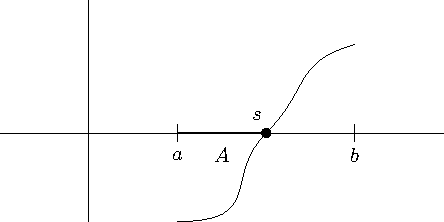
\includegraphics{chapter3/images/zwischen}
  \caption{Zwischenwertsatz}%
  \label{fig:zwischen}
\end{figure}

\subsection*{Folgerungen}
\begin{zwischenwertsatz}
  Sei $f \colon [a, b] \to \mathbb{R} $
  stetig mit $f(a) \leq f(b)$.
  Dann gilt 
  \[[f(a), f(b)] \subset f([a, b]).\]
\end{zwischenwertsatz}

\begin{proof}
  Sei $y \in [f(a), f(b)]$. Betrachte
  auf $[a, b]$ die stetige Funktion
  $g(x) = f(x) - y$.
  Es gilt $g(a) = f(a) - y \leq 0$ und
  $g(b) = f(b) - y \geq 0$.
  Also existiert nach Theorem~\ref{thm:pre-zwischen}
  ein Punkt $p \in [a, b]$ mit $g(p) = 0$,
  beziehungsweise $f(p) = y$.
\end{proof}

\begin{example}
  Seien $a_1, a_2, \dots, a_{2k + 1} \in \mathbb{R}$.
  Setze
  \[
  f(x) = x^{2k+1} + a_1 x^{2k}
  + \cdots + a_{2k}x + a_{2k+1}.
  \]
  Dann ist $f$ ein \emph{Polynom} von ungeradem
  \emph{Grad} $2k + 1$. Es gilt
  \[
    \lim_{n \to \infty} \frac{f(n)}{n^{2k+1}}
    = \lim_{n \to \infty}
    \left( 1 + \frac{a_1}{n} + \frac{a_2}{n^2}
    + \cdots + \frac{a_{2k+1}}{n^{2k+1}}\right) = 1.
  \]
  Folglich nimmt $f$ beliebig hohe Werte an.
  Ähnlich gilt
  \[
    \lim_{n \to \infty} \frac{f(-n)}{n^{2k+1}}
    = \lim_{n \to \infty}
    \left( -1 + \frac{a_1}{n} - \frac{a_2}{n^2}
    + \cdots + \frac{a_{2k+1}}{n^{2k+1}}\right) = -1,
  \]
  also nimmt $f$ negative Werte
  mit beliebig hohem Betrag an.
  Nach dem Zwischenwertsatz 
  ist $f$ surjektiv, insbesondere hat $f$ eine Nullstelle.
\end{example}

\begin{remark}
  Für Polynome mit geradem Grad ist das falsch:
  Die Funktion $f(x) = x^2 + 1$ hat keine Nullstelle
  in $\mathbb{R}$.
\end{remark}

\begin{brouwer}
  Sei $f \colon [a, b] \to [a, b]$ stetig.
  Dann existiert $p \in [a, b]$ mit $f(p) = p$.
\end{brouwer}

Ein solcher Punkt $p$ mit $f(p) = p$ heisst \emph{Fixpunkt}
von $f$.

\begin{proof}
  Betrachte die auf dem Intervall
  $[a, b]$ stetige Funktion
  $g(x) = x - f(x)$.
  Es gilt
  $
    g(a) = a - f(a) \leq 0$
    und
    $g(b) = b - f(b) \geq 0$.
  Nach dem Zwischenwertsatz existiert
  $p \in [a,b]$ mit $g(p) = 0$,
  beziehungsweise $f(p) = p$.
\end{proof}

\begin{figure}[htb]
  \centering
  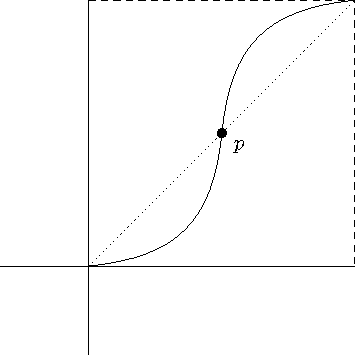
\includegraphics{chapter3/images/brouwer}
  %TODO
  \caption{Fixpunktsatz von Brouwer.
  Ein Schnittpunkt des Graphen von $f$ mit
der Gerade mit Steigung $1$ ist ein
Fixpunkt von $f$. Die eingezeichnete Abbildung
hat sogar drei Fixpunkte, zum Beispiel $p$.}%
  \label{fig:brouwer}
\end{figure}

\section{Stetige Funktionen auf kompakten Mengen}

\begin{question}
Sei $A \subset \mathbb{R}$ beschränkt,
das heisst es existiert $R > 0$ 
mit $A \subset [-R, R]$.
Sei $f \colon A \to \mathbb{R}$ stetig.
Ist dann $f(A) \subset \mathbb{R}$ beschränkt?
\end{question}

\begin{example}
  Die Antwort ist nein. Sei 
  \[
    A = (0, 1) = \left\{x \in \mathbb{R} \mid 0 < x < 1\right\}
  \]
  und $f(x) = 1/x$. Dann ist $f((0, 1)) = \mathbb{R}_{>0}$ 
  unbeschränkt.
\end{example}

\begin{definition}
  Eine Teilmenge
  $U \subset \mathbb{R}$ 
  heisst \emph{offen},
  falls für
  alle $p \in U$ ein
  $\delta > 0$ existiert,
  so dass $(p - \delta, p + \delta)
  \subset U$.
Eine Teilmenge
  $A \subset \mathbb{R}$ 
  heisst  \emph{abgeschlossen},
  falls $\mathbb{R} \setminus A$ 
  offen ist.
\end{definition}

\begin{remark}
  Jede (auch unendliche) Vereinigung offener Mengen ist offen
  (aber unendliche Vereinigungen abgeschlossener Mengen
  sind nicht unbedingt abgeschlossen).
\end{remark}

\begin{examples}
  \leavevmode
  \begin{itemize}
    \item Sei
      $a < b$. Dann ist
      das \emph{offene Intervall}
      \[
        U = (a, b) = \left\{x \in \mathbb{R} \mid a < x < b\right\}
      \]
      zwischen $a$ und $b$ offen. Sei dazu $p \in (a, b)$. Setze
      $\delta = \min \{|p - a|, |p - b|\}$.
      Dann gilt
      $(p - \delta, p + \delta) \subset (a, b)$,
      siehe Abbildung~\ref{fig:offen}.
      \begin{figure}[htb]
        \centering
        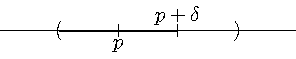
\includegraphics{chapter3/images/offen}
        \caption{Offene Intervalle
        sind offen}%
        \label{fig:offen}
      \end{figure}
      
    \item Sei $a \leq b$. Dann ist das \emph{abgeschlossene Intervall}
      \[
        A = [a, b] = \left\{x \in \mathbb{R} \mid a \leq x \leq b\right\}
      \]
      zwischen $a$ und $b$ abgeschlossen.
      Sei dazu $p \notin [a,b]$, das heisst entweder
      $p < a$ oder $p > b$.
      Setze $\delta = \min \{|p- a|, |p-b|\} > 0$.
      Dann gilt
      $(p - \delta, p + \delta) \cap [a, b] = \emptyset$,
      also ist $\mathbb{R} \setminus [a, b]$ offen.
    \item Sei $A = \{0\} \cup \left\{1/n \mid n \in 
      \mathbb{N}, n \geq 1\right\}$.
      Dann ist $A$ abgeschlossen, da
      \[
        \mathbb{R} \setminus A = \mathbb{R}_{<0} \cup
        \mathbb{R}_{>1} \cup \bigcup_{n \in \mathbb{N}_{\geq 1}}
        \left(/1(n+1), 1/n\right)
      \]
      eine Vereinigung offener Mengen und somit selbst offen ist.
    \item Die Menge
      \[
        B = \left\{1/n \mid n \in \mathbb{N}, n \geq 1\right\}
      \]
      ist weder offen noch abgeschlossen.
    \item Die Menge $\mathbb{Q} \subset \mathbb{R}$ 
      ist weder offen noch abgeschlossen.
    \item Die Menge
      \[
        [0, 1) = \left\{x \in \mathbb{R} \mid 0 \leq%chktex 9
        x < 1\right\}
      \]
      ist weder offen noch abgeschlossen.
  \end{itemize}
\end{examples}

\begin{theorem}\label{thm:extreme}
  Sei $A \subset \mathbb{R}$ abgeschlossen
  und beschränkt,
  und sei weiterhin $f \colon A \to \mathbb{R}$
  stetig. Dann nimmt $f$ auf $A$ ein
  Maximum und ein Minimum an,
  das heisst es existiert $p \in A$,
  so dass für alle $q \in A$ gilt,
  dass $f(q) \leq f(p)$, beziehungsweise $f(q) \geq f(p)$.
\end{theorem}

Für den Beweis von Theorem~\ref{thm:extreme}
brauchen wir noch etwas Vorarbeit.

\begin{lemma*}
  Sei $A \subset \mathbb{R}$ abgeschlossen
  und $a \colon \mathbb{N} \to A$ eine konvergente
  Folge. Dann liegt der
  Grenzwert $\lim_{n \to \infty} a_n$ in $A$.
\end{lemma*}

\begin{proof}
  Wir beweisen das Lemma durch Widerspruch.
  Sei
  \[
    p = \lim_{n \to \infty} a_n \in \mathbb{R} \setminus A.
  \]
  Da $\mathbb{R} \setminus A$ offen ist,
  existiert $\delta > 0$ mit $(p - \delta, p + \delta)
  \subset \mathbb{R} \setminus A$.
  Wähle $N \in \mathbb{N}$  so dass für alle $n \geq N$
  gilt, dass $|a_n - p| < \delta$.
  Aber dann gilt $a_n \in (p - \delta, p + \delta)
  \subset \mathbb{R} \setminus A$,
  also $a_n \notin A$, was der Annahme, dass 
  $a \colon \mathbb{N} \to A$
  eine Folge in $A$ ist, widerspricht.
\end{proof}




\end{document}
